\jxhj{%教学后记
	}
\skrq{%授课日期
	2017年12月12日 4-5节}
\ktmq{%课题名称
	 Siemens上的长度补偿}
\jxmb{%教学目标,每行前面要加 \item
	\item 掌握Siemens上的换刀指令;
\item 掌握Siemens上的长度补偿;
\item 掌握Siemens长度补偿编程。}
\jxzd{%教学重点,每行前面要加 \item
	\item Siemens上的长度补偿;
	\item 掌握加工中心编程。 }
\jxnd{%教学难点,每行前面要加 \item
	\item Siemens上的长度补偿。 }
\jjff{%教学方法
	通过讲述、举例、演示法来说明;}

\makeshouye %制作教案首页

%%%%教学内容
\subsection{组织教学}
\begin{enumerate}[\hspace{2em}1、]
\item 集中学生注意力;
\item 清查学生人数;
\item 维持课堂纪律;
\end{enumerate}

\subsection{复习导入及主要内容}
\begin{enumerate}[1、]
\item Fanuc长度补偿的执行过程;
\item 安全使用长度补偿;
\item 三种补偿值的比较;
\item 编程实例。
\end{enumerate}

\subsection{教学内容及过程}

\subsubsection{Siemen上的换刀}
M5

TnD1

M3……

此语句包括换刀及刀具长度补偿

补偿值的确定与Fanuc中的G43指令中的长度补偿值的确定一样。

基准刀: 补偿长度为0

其它刀具:待测刀长-基准刀长

(有正有负)

\subsubsection{加工实例}

在Siemens的加工中心上加工如图所示的零件。完成工艺分及加工程序的编写:


\begin{figure}[h]
	\centering
	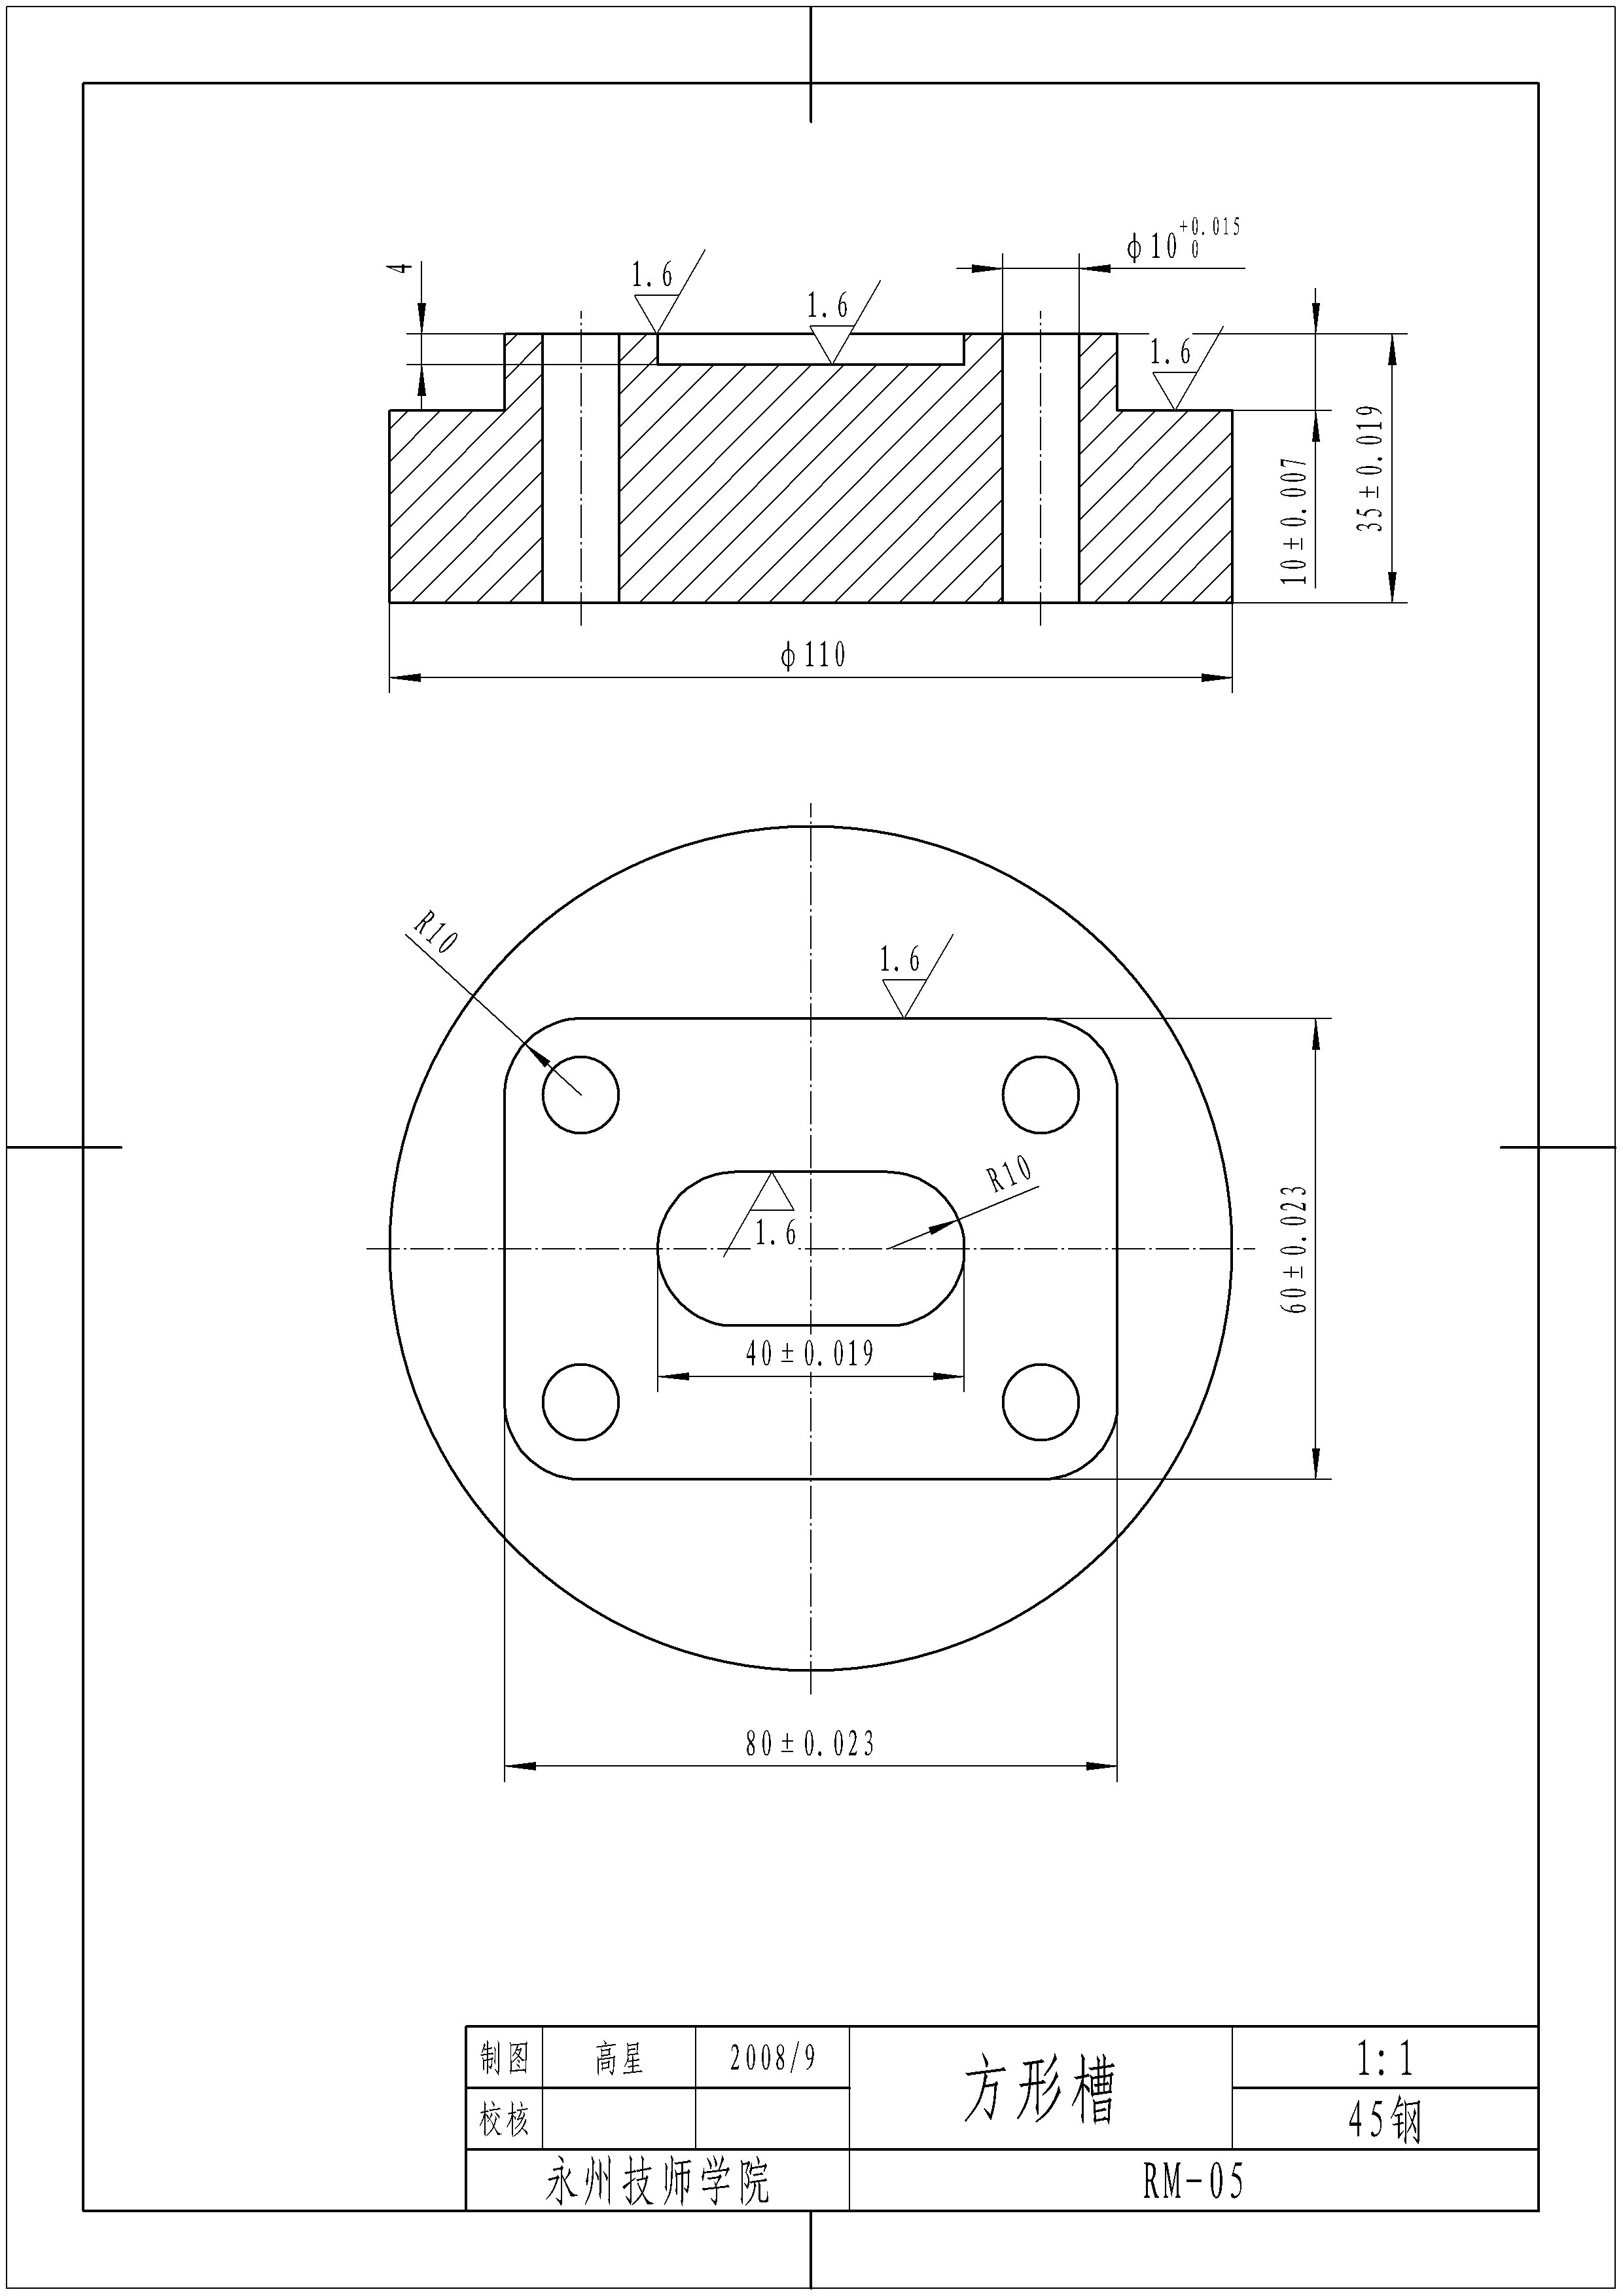
\includegraphics[width=0.7\linewidth]{data/image/26-1}
	\caption{实例}
	\label{fig:26-1}
\end{figure}


1、工件坐标系:工件上表面的中心(面铣后的上表面)

2、装夹:卡盘或平口钳(在两侧加工安装侧面)

3、刀具:

$\varnothing$16三齿立铣刀:面铣、粗加工内外轮廓

$\varnothing$12立铣发:精加工内外轮廓

$\varnothing$5中心钻:钻中心孔

$\varnothing$9.8麻花钻:钻孔

$\varnothing$10机用铰刀:铰孔

4、工序表:

如表\ref{biao:1}

\begin{table}[h]
	\centering
	\caption[表]{工序表}
	\label{biao:1}
\begin{tabular}{|c|c|c|c|c|c|c|}
	\hline 
	1&铣上表面&φ16立铣刀&T1D1&400&200&无\\ 
	\hline 
	2&粗铣外轮廓&φ16立铣刀&T1D1&400&200&\\ 
	\hline
	3&粗铣槽&φ16立铣刀&T1D1&400&200&\\ 
	\hline
	4&钻中心孔&φ5中心钻&T3D1&1200&80&无\\ 
	\hline
	5&钻孔&φ9.8头&T4D1&500&60&无\\ 
	\hline
	6&铰孔&φ10铰刀&T5D1&200&30&无\\ 
	\hline
	7&精铣外轮廓&φ12立铣刀&T2D1&800&120&\\ 
	\hline 
\end{tabular} 
\end{table}

5、走刀路径及相关点坐标

A、面铣: 

B、加工外外轮廓: 

C、内轮廓加工:Z字形下刀。

D:孔加工:

6、参考程序:

\begin{lstlisting}
GX_01(主程序)
G54G17G40G90
T1D1(换16立铣刀)
L11
T3D1(换5中心钻)
L33
T4D1(换9.8钻头)
L41
T5D1(换10铰刀)
L51
T2D1(换12立铣)
L21
M5
\end{lstlisting}


\subsection{课堂小结}
\begin{enumerate}[1、]
\item Siemens 上的换刀;
\item Simens上的长度补偿;
\item 编程实例。
\end{enumerate}

\vfill
\subsection{布置作业}
\begin{enumerate}[1、]
\item 综合习题一。
\end{enumerate}
\vfill